\documentclass[a4paper,10pt]{article} 
\usepackage[utf8]{inputenc}
\usepackage[a4paper]{geometry}
\usepackage[magyar]{babel}
\usepackage{t1enc}
\usepackage{amsmath}
\usepackage{amssymb}
\usepackage{caption}
\usepackage{pgf,tikz}
\frenchspacing 
\pagestyle{empty}
\newcommand{\ki}[2]{\hfill {\it #1 (#2)}\medskip}
\newcommand{\vonal}{\hbox to \hsize{\hskip2truecm\hrulefill\hskip2truecm}}
\newcommand{\degre}{\ensuremath{^\circ}}
\newcommand{\tg}{\mathop{\mathrm{tg}}\nolimits}
\newcommand{\ctg}{\mathop{\mathrm{ctg}}\nolimits}
\newcommand{\arc}{\mathop{\mathrm{arc}}\nolimits}
\renewcommand{\vec}[1]{\mathbf{#1}}
\begin{document}
\begin{center} \Large {\em XXII. Nemzetközi Magyar Matematikaverseny} \end{center}
\begin{center} \large{\em Győr, 2013. március 14--18.} \end{center}
\smallskip
\begin{center} \large{\bf 11. osztály} \end{center}
\bigskip

{\bf 1. feladat: } Oldja meg a valós számok halmazán a következő egyenletet:
\[x+\frac{x}{x-1}+\frac{x^2}{x^2-x+1}=\frac{49}{6}\]

\ki{Kovács Béla}{Erdély}\medskip

{\bf I. megoldás: } Az egyenlet értelmezési tartománya az $\mathbb{R}\setminus{1}$ halmaz; $x^2-x+1>0$ minden valós $x$-re.

Legyen $x+\frac{x}{x-1}=\frac{x^2}{x-1}=t$. Az új ismeretlennel felírhatjuk a harmadik tagot is:
\[\frac{x^2}{x^2-x+1}=\frac{\frac{x^2}{x-1}}{\frac{x^2}{x-1}-1}=\frac{t}{t-1}.\]

Így az egyenlet:
\[t+\frac{t}{t-1}=\frac{49}{6}.\]

Felszorzunk és rendezünk.
\[6t^2-49t+49=0\]
A másodfokú egyenlet gyökei $t_1=7$ és $t_2=\frac{7}{6}$.

Visszatérünk a helyettesítéshez.

\[t_1=\frac{x^2}{x-1}=7 \implies x^2-7x+7=0\]
Ezen másodfokú egyenlet gyökei
\[x_{1,2}=\frac{7\pm\sqrt{21}}{2}.\]

\[t_2=\frac{x^2}{x-1}=\frac{7}{6} \implies 6x^2-7x+7=0\]
Ez utóbbi másodfokú egyenletnek nincs valós gyöke.

Tehát az eredeti egyenlet valós megoldásai:
\[x_{1,2}=\frac{7\pm\sqrt{21}}{2}.\]
\medskip

{\bf II. megoldás: } Közös nevezőre való hozással és átalakításokkal rendezve az egyenlet:
\[x^4-49x^3+98x^2-98x+49=0.\]
Szorzattá alakíthatunk:
\[\left(x^2-7x+7\right)\left(6x^2-7x+7\right)=0.\]
Egy szorzat akkor és csak akkor nulla, ha valamelyik tényezője nulla -- a két másodfokú egyenlet megoldása után kapjuk az eredeti egyenlet gyökeit.
\medskip

\vonal
{\bf 2. feladat: } Az $x$, $y$, $z$ valós számok eleget tesznek az
\[x^2+3y^2+z^2=2\]
egyenletnek. Mekkora lehet a $2x+y-z$ kifejezés legnagyobb értéke és mely $x$, $y$, $z$
számokra veszi ezt fel?

\ki{Pintér Ferenc}{Magyarország}\medskip

{\bf I. megoldás: } Legyen $2x+y-z=t$, ahonnan $z=2x+y-t$, melyet helyettesítsünk be a feltétel egyenletébe. Ekkor a következőhöz jutunk:
\[x^2+3y^2+(2x+y-t)^2=2.\]
Végezzük el a műveleteket és rendezzünk $x$ hatványai szerint.
\[5x^2+4(y-t)x+4y^2-2ty+t^2-2=0\]

Ez $x$-ben másodfokú egyenlet -- $x$-re valós gyököt csak akkor kaphatunk, ha az egyenlet diszkriminánsa nemnegatív.
\begin{align*}
D=16(y-t)^2-4\cdot5\left(4y^2-2ty+t^2-2\right)&\ge0\\
4(y-t)^2-5\left(4y^2-2ty+t^2-2\right)&\ge0\\
4y^2-8ty+4t^2-20y^2+10ty-5t^2+10&\ge0\\
0&\ge16y^2-2ty+t^2-10
\end{align*}
Ennek az egyenlőtlenségnek akkor van megoldása, ha bal oldalon álló $y$-ban másodfokú kifejezésnek van zérushelye, vagyis ha a diszkriminánsa nem kisebb nullánál:
\begin{align*}
4t^2-4\cdot16\cdot\left(t^2-10\right)&\ge0\\
t^2-16t^2+160&\ge0\\
160\ge15t^2\\
\frac{32}{3}\ge t^2
\end{align*}
Ebből az egyenlőtlenségből megkapjuk $t$ legnagyobb értékét:
\[t_{\max}=\sqrt\frac{32}{3}.\]

Innen az előző egyenlőtlenségekben mindenütt egyenlőséget írva és behelyettesítve $t$ maximális értékét, visszafelé haladva kapjuk $y$, $x$ és $z$ azon értékét, ahol $t$ felveszi maximumát:
\[x=\sqrt\frac32,\quad y=\frac16\sqrt\frac32,\quad z=-\frac12\sqrt\frac32.\]
Ezen értékek valóban kielégítik az eredeti feltételt: 
\[\left(\sqrt\frac32\right)^2+3\left(\frac16\sqrt\frac32\right)^2+ \left(-\frac12\sqrt\frac32\right)^2=
\frac32+3\cdot\frac{1}{36}\cdot\frac32+\frac14\cdot\frac32=2.\]

\medskip

{\bf II. megoldás: } Legyen $2x+y-z=t$, és ennek valamilyen pozitív $\alpha$-szorosát vonjuk ki a feltétel egyenletéből, majd rendezzünk.
\begin{align*}
x^2+3y^2-z^2-2\alpha x-\alpha y+\alpha z&=2-\alpha t\\
(x-\alpha)^2-\alpha^2+\left(\sqrt3y-\frac{\alpha}{2\sqrt3}\right)^2-\frac{\alpha^2}{12}+\left(z+\frac{\alpha}{2}\right)^2-\frac{\alpha^2}{4}&=2-\alpha t\\
(x-\alpha)^2+\left(\sqrt3y-\frac{\alpha}{2\sqrt3}\right)^2+\left(z+\frac{\alpha}{2}\right)^2&=2-\alpha t+\frac43\alpha^2
\end{align*}
Tudjuk, hogy a bal oldal nemnegatív, így a jobb oldal is az. Mivel célunk $t$ maximalizálása, ez azt jelenti, hogy mindkét oldal 0. Ekkor
\[0=2-\alpha t+\frac43\alpha^2 \iff t=\frac{2}{\alpha}+\frac{4}{3}\alpha,\]
felhasználva, hogy $\alpha$ pozitív. A bal oldal pontosan akkor nulla, ha minden tag nulla. Ez akkor teljesül, ha
\[x=\alpha,\quad y=\frac{\alpha}{6},\quad z=-\frac{\alpha}{2}.\]

Az $x$-re, $y$-ra és $z$-re kapott értékeket visszaírva a feltételbe megkapjuk a maximális $t$-hez tartozó $\alpha$ értékét.
\begin{align*}
\alpha^2+3\left(\frac{\alpha}{6}\right)^2+\left(\frac{\alpha}{2}\right)^2&=2\\
\alpha^2+\frac{\alpha^2}{12}+\frac{\alpha^2}{4}&=2\\
\frac43\alpha^2&=2\\
\alpha&=\sqrt\frac32.
\end{align*}

Válasszuk meg tehát így $\alpha$-t. A fenti levezetésből már kiderül, hogy $t$ akkor veszi fel maximális értékét, ha
\[x=\sqrt\frac32,\quad y=\frac16\sqrt\frac32,\quad z=-\frac12\sqrt\frac32.\]
A maximális érték tehát
\[t_{\max}=\frac{2}{\alpha}+\frac43\alpha=\sqrt\frac{32}{3}.\]

\medskip

{\bf III. megoldás: } Tekintsük az $\vec{u}\left(x;\sqrt3y;z\right)$ és $\vec{v}\left(2;\frac{1}{\sqrt3};-1\right)$ vektorokat, az általuk bezárt szög legyen $\varphi$.

A vektorok abszolút értékei
\[|\vec{u}|=\sqrt{x^2+3y^2+z^2}=\sqrt2\quad\text{és}\quad|\vec{v}|\sqrt{4+\frac13+1}=\frac{4}{\sqrt3},\]
skaláris szorzatuk
\[\vec{u}\vec{v}=2x+y-z.\]

A Cauchy--Schwarz--Bunyakovszkij-egyenlőtlenség szerint $\vec{u}\vec{v}\le|\vec{u}|\cdot|\vec{v}|$, és egyenlőség akkor és csak akkor teljesül, ha a két vektor lineárisan összefüggő, azaz ha $\vec{u}=\lambda\vec{v}$, tehát
\[x=2\lambda,\quad y=\frac{\lambda}{3},\quad z=-\lambda.\]

Így kifejezhetjük $x$-szel a másik két változót: $y=\frac16x$, $z=-\frac12x$. Ezt visszaírva a feltételbe megkapjuk $x$ értékét.
\begin{align*}
x^2+3\left(\frac{x}{6}\right)^2+\left(-\frac{x}{2}\right)^2&=2\\
x^2+\frac{x^2}{12}+\frac{x^2}{4}&=2\\
\frac{4x^2}{3}&=2\\
x^2&=\frac{3}{2}
\end{align*}

$x=\sqrt\frac32$-re $y=\frac16\sqrt\frac32$ és $z=-\frac12\sqrt\frac32$; $x=-\sqrt\frac32$-re $y=-\frac16\sqrt\frac32$ és $z=\frac12\sqrt\frac32$ -- utóbbi esetben $2x+y-z$ negatív, így ez nem ad maximumot. Az előbbi esetben
\[2x+y-z=2\sqrt\frac32+\frac16\sqrt\frac32+\frac12\sqrt\frac32=\frac83\sqrt\frac32=\frac{4\sqrt2}{\sqrt3}=\sqrt{\frac{32}{3}},\]
ami valóban $|\vec{u}|$ és $|\vec{v}|$ szorzata. A kifejezés legnagyobb értéke tehát $\sqrt{\frac{32}{3}}$, amit a megadott $x$, $y$, $z$ értékekre fel is vesz.

\medskip

\vonal
{\bf 3. feladat: } Mutassa meg, hogy a következő egyenletnek nincs megoldása az $(x; y)$ pozitív egész számpárok halmazán:
\[(3x+3y)^2+12x+12y=8048+(x-y)^2.\]

\ki{Nemecskó István}{Magyarország}\medskip

{\bf Megoldás: } Mindkét oldalhoz 4-et adunk és rendezünk:
\begin{align*}
(3x+3y)^2+4(3x+3y)+4-(x-y)^2&=8052\\
(3x+3y+2)^2-(x-y)^2&=8052\\
(2x+y+1)(x+2y+1)&=2013\\
\end{align*}

Ha $x$ és $y$ pozitív egész számok, akkor a zárójelben álló kifejezések is azok. Felírjuk 2013 prímtényezős felbontását:
\[(2x+y+1)(x+2y+1)=3\cdot11\cdot61\]

Legyen tehát
\begin{align*}
2x+y+1&=d_1,\\
x+2y+1&=d_2,
\end{align*}
ahol $d_1\cdot d_2=2013$.

Kifejezzük $x$-et és $y$-t:
\begin{align*}
3y&=2d_2-d_1-1,\\
3x&=2d_1-d_2-1.
\end{align*}

$x$ és $y$ szerepe szimmetrikus, így feltehetjük, hogy $d_1>d_2$ ($d_1\ne d_2$, mert 2013 nem négyzetszám).

A lehetséges felbontásokat a táblázat mutatja: az első három esetben $y$ jól láthatóan negatív lesz, a negyedik esetben pedig nem egész szám:
\[
\begin{array}{ccc}
d_1 & d_2 & y\\
\hline
2013 & 1 & \textrm{negatív}\\
671 & 3 & \textrm{negatív}\\
183 & 11 & \textrm{negatív}\\
61 & 33 & \frac{2\cdot33-61-1}{3}=\frac43 
\end{array}
\]

Ezzel bebizonyítottuk, hogy az egyenletnek nincs megoldása a pozitív egész számpárok halmazán.

{\it Megjegyzés: } az egészek halmazán az egyenletnek nyolc megoldása van:
\[\begin{array}{cccc}
(-1342; 670), &(-222; 446), &(-54; 118), &(-30; -2),\\
(670; -1342), &(446; -222), &(118; -54), &(-2; -30).
\end{array}\]

\medskip

\vonal
{\bf 4. feladat: } Tekintsünk egy $5\times5$-ös méretű ,,sakktáblát''. Jelentse az adott sakktábla egy kitöltését az az eljárás, melynek során minden mezőbe beírunk pontosan egyet az 1, 2, 3, \ldots{} 25 számok közül. Adja meg a fenti sakktáblának egy olyan kitöltését, melyben a számok soronkénti összegeinek szorzata a lehető legnagyobb.

\ki{Bíró Béla}{Erdély}\medskip

{\bf Megoldás: } A feladatban megfogalmazott feltételek mellett az adott sakktáblát véges sokféleképpen tölthetjük ki (összesen $25!$-féle kitöltés van, ha a szimmetrikus kitöltéseket nem tekintjük azonosnak). Minden kitöltéshez tartozik a soronkénti számok összegeinek egy-egy szorzata. Tehát ezen szorzatszámok halmaza is véges, ezért van közöttük legnagyobb.

Jelöljük a soronkénti számok változó összegszámait $a$, $b$, $c$, $d$, $e$-vel. A számtani és mértani közepek közti egyenlőtlenség felhasználásával írhatjuk, hogy:
\[abcde\le\left(\frac{a+b+c+d+e}{5}\right)^5=\left(\frac{325}{5}\right)^5=65^5,\]
mert $a+b+c+d+e=1+2+\ldots+25=325$. Egyenlőség pontosan akkor áll fenn, ha $a=b=c=d=e=65$.

Megvalósítható olyan kitöltés, ahol ez a feltétel teljesül, tehát ahol a soronkénti összegek egyenként 65-tel egyenlők: egy ilyen kitöltést mutat a táblázat.

%\begin{table}
\begin{center}
\begin{tabular}{|c|c|c|c|c|}
\hline
11&12&13&14&15\\
\hline
4&10&16&17&18\\
\hline
2&3&19&20&21\\
\hline
5&7&8&22&23\\
\hline
1&6&9&24&25\\
\hline
\end{tabular}
\end{center}
%\caption*{A 4.~feladathoz.}
%\end{table}

A szorzat maximuma tehát $65^5$, amelyet a bemutatott kitöltés esetén meg is valósul.

\medskip

\vonal
{\bf 5. feladat: } Legyen az $ABC$ háromszög $AB$ oldalának belső pontja $P$. Az $AC$ egyenest az $A$ pontban érintő, illetve a $BC$ egyenest a $B$ pontban érintő körök metszéspontjai a $P$ és $Q$ pontok. Bizonyítsa, hogy a $C$ pontnak az $AB$ szakasz felezőmerőlegesére vonatkozó tükörképe illeszkedik a $PQ$ egyenesre!

\ki{Bíró Bálint}{Magyarország}\medskip

{\bf Megoldás: } Legyen az $ABC$ háromszög köré írt kör $k$.

Először azt fogjuk bizonyítani, hogy a $Q$ pont rajta van $k$-n.

A $k_1$ kör az $A$ pontban érinti az $AC$ egyenesét, hasonlóképpen a $k_2$ kör a $B$ pontban érinti a $BC$ egyenesét. Az érintő tulajdonsága és a kerületi szögek tétele miatt $PAC\sphericalangle=PQA\sphericalangle$ -- ezek a $Q$ pontot
nem tartalmazó $AP$ körívhez tartozó kerületi szögek a $k_1$ körben --, ugyanígy
$PBC\sphericalangle=PQB\sphericalangle$ -- ezek a szögek a $Q$ pontot nem tartalmazó $BP$ körívhez tartozó kerületi szögek a $k_2$ körben. Nyilvánvalóan $PAC\sphericalangle=BAC\sphericalangle$ és $PBC\sphericalangle=ABC\sphericalangle$.

\begin{figure}[htb]
\begin{center}
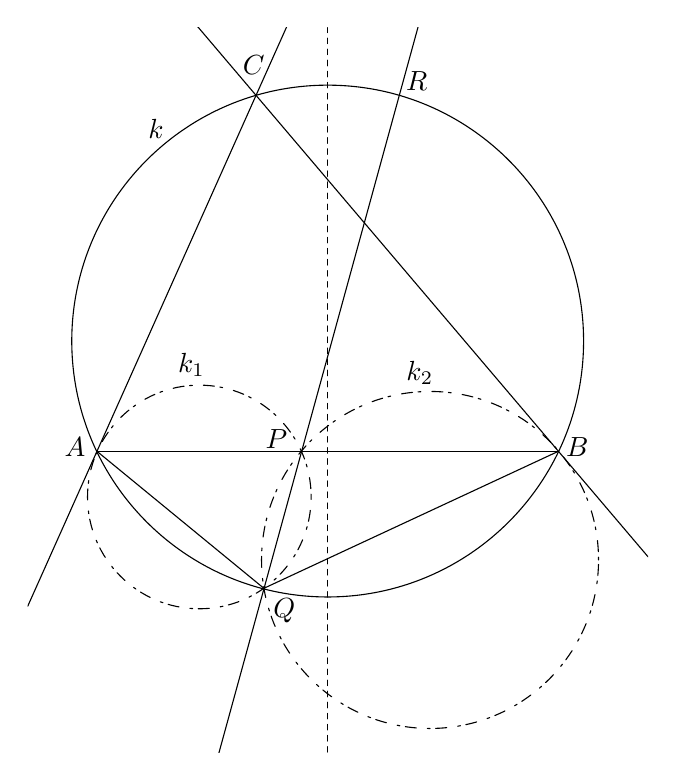
\begin{tikzpicture}[line cap=round,line join=round,x=1.0cm,y=1.0cm]
\clip(-0.88,-3.82) rectangle (7,5.38);
\draw(2.93,1.4) circle (3.25cm);
\draw [dash pattern=on 2pt off 2pt] (2.93,-3.82) -- (2.93,5.38);
\draw [domain=-0.88:7] plot(\x,{(--11.75-4.52*\x)/-1.24});
\draw [dash pattern=on 1pt off 2pt on 4pt off 4pt] (1.3,-0.58) circle (1.42cm);
\draw [dash pattern=on 1pt off 2pt on 4pt off 4pt] (4.23,-1.38) circle (2.14cm);
\draw [domain=-0.88:7] plot(\x,{(-0--4.52*\x)/2.02});
\draw [domain=-0.88:7] plot(\x,{(--26.49-4.52*\x)/3.84});
\draw (5.86,0)-- (0,0);
\draw (2.12,-1.74)-- (0,0);
\draw (2.12,-1.74)-- (5.86,0);
%\draw [fill=black] (0,0) circle (1.5pt);
\draw[color=black] (-0.28,0.05) node {$A$};
%\draw [fill=black] (5.86,0) circle (1.5pt);
\draw[color=black] (6.1,0.05) node {$B$};
%\draw [fill=black] (2.02,4.52) circle (1.5pt);
\draw[color=black] (1.99,4.91) node {$C$};
\draw[color=black] (.75,4.1) node {$k$};
%\draw [fill=black] (2.6,0) circle (1.5pt);
\draw[color=black] (2.28,0.16) node {$P$};
%\draw [fill=black] (3.84,4.52) circle (1.5pt);
\draw[color=black] (4.06,4.7) node {$R$};
%\draw [fill=black] (2.12,-1.74) circle (1.5pt);
\draw[color=black] (2.38,-2.02) node {$Q$};
\draw[color=black] (1.2,1.1) node {$k_1$};
\draw[color=black] (4.1,1.) node {$k_2$};
\end{tikzpicture}
\end{center}
\caption*{Az 5. feladathoz.}
\end{figure}

Ezek szerint
\[BAC\sphericalangle+ABC\sphericalangle=PQA\sphericalangle+PQB\sphericalangle= AQB\sphericalangle=180^\circ-ACB\sphericalangle,\]
azaz az $AQBC$ négyszög két szemközti szögének összege $180^\circ$, tehát a négyszög húrnégyszög, így $Q$ rajta van a $k$ körön. (A $C$ és $Q$ pontok az $AB$ egyenes különböző oldalán vannak).

Legyen most a $PQ$ egyenes és a $k$ kör $Q$-tól különböző metszéspontja $R$. Azt fogjuk bizonyítani, hogy a $C$ pontnak az $AB$ szakasz felezőmerőlegesére vonatkozó tükörképe éppen az $R$ pont.

Az előzőek szerint $BAC\sphericalangle=PQA\sphericalangle=RQA\sphericalangle$, ugyanakkor $k$-ban egyenlő nagyságú kerületi szögekhez egyenlő hosszúságú húrok tartoznak, tehát $BC=AR$.

Hasonlóképpen igazolható, hogy $ABC\sphericalangle=PQB\sphericalangle=RQB\sphericalangle$ miatt $AC=BR$.

Ezért az $R$ pont az $A$ és $B$ pontoktól rendre $BC$, illetve $AC$ távolságra van, ez pedig csak úgy lehetséges, hogy az $R$ pont nem más, mint a $C$ pontnak az $AB$ szakasz felezőmerőlegesére vonatkozó tükörképe. Ezzel a feladat állítását bizonyítottuk.

{\it Megjegyzés. } A feladat eredménye az is, hogy rögzített $A$, $B$, $C$ pontok mellett a $C$ pontnak az $AB$ szakasz felezőmerőlegesére vonatkozó tükörképe mindig ugyanaz az $R$ pont, és a $P$ pont $AB$ szakaszon belül elfoglalt helyzetétől függetlenül a $PQ$ egyenes mindig az $R$ ponton megy át.

{\it Megjegyzés. } A feladat állítása már az $BAC\sphericalangle=PQA\sphericalangle=RQA\sphericalangle$ egyenlőségből következik, mert eszerint $\widehat{BC}=\widehat{AR}$, ami miatt $ABRC$ húrtrapéz.

\medskip

\vonal
{\bf 6. feladat: } Jelöljük az $ABC$ háromszög szögeit $\alpha$, $\beta$, $\gamma$-val, az említett szögekkel szemközti oldalakat pedig rendre $a$, $b$, $c$-vel. Bizonyítsa be, hogy $b<\frac{1}{2}(a+c)$ esetén $\beta<\frac{1}{2}(\alpha+\gamma)$.

\ki{Fonyó Lajos}{Magyarország}\medskip

{\bf I. megoldás: } Hosszabbítsuk meg az $ABC\triangle$ $BA$ és $BC$ oldalait $A$-n és $C$ túl rendre $a$, illetve $c$ távolsággal; legyenek a kapott pontok $D$ és $E$.

$BD=BE=a+c$, tehát $BDE$ egyenlő szárú háromszög. Húzzunk $D$-n keresztül $AC$-vel, $C$-n keresztül $AD$-vel párhuzamost, ezek metszéspontja legyen $F$. $DFCA$ paralelogramma a párhuzamosságok miatt: $FC=DA=a$ és $DF=AC=b$.

\begin{figure}[hbt]
\begin{center}
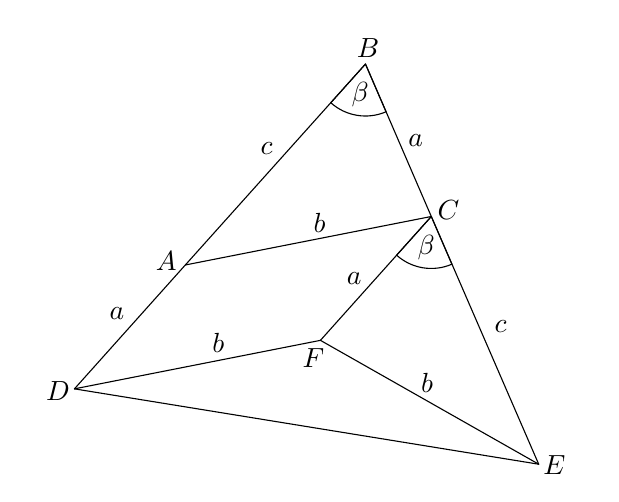
\begin{tikzpicture}[line cap=round,line join=round,x=1.1cm,y=1.1cm]
\clip(-0.78,1.45) rectangle (5.72,6.6);
\draw [shift={(3.12,6.18)}] (0,0) -- (-131.88:0.6) arc (-131.88:-66.64:0.6) -- cycle;
\draw [shift={(3.88,4.42)}] (0,0) -- (-131.88:0.6) arc (-131.88:-66.64:0.6) -- cycle;
\draw (1.04,3.86)-- (3.88,4.42);
\draw (3.12,6.18)-- (3.88,4.42);
\draw (3.88,4.42)-- (5.12,1.56);
\draw (-0.24,2.43)-- (5.12,1.56);
\draw (-0.24,2.43)-- (1.04,3.86);
\draw (1.04,3.86)-- (3.12,6.18);
\draw (3.88,4.42)-- (2.6,2.99);
\draw (2.6,2.99)-- (5.12,1.56);
\draw (2.6,2.99)-- (-0.24,2.43);
%\draw [fill=black] (1.04,3.86) circle (1.5pt);
\draw[color=black] (0.82,3.9) node {$A$};
%\draw [fill=black] (3.12,6.18) circle (1.5pt);
\draw[color=black] (3.15,6.37) node {$B$};
%\draw [fill=black] (3.88,4.42) circle (1.5pt);
\draw[color=black] (4.08,4.5) node {$C$};
%\draw [fill=black] (-0.24,2.43) circle (1.5pt);
\draw[color=black] (-0.43,2.4) node {$D$};
%\draw [fill=black] (5.12,1.56) circle (1.5pt);
\draw[color=black] (5.3,1.55) node {$E$};
\draw[color=black] (2.59,4.35) node {$b$};
\draw[color=black] (3.7,5.3) node {$a$};
\draw[color=black] (4.68,3.15) node {$c$};
\draw[color=black] (0.25,3.3) node {$a$};
\draw[color=black] (1.98,5.2) node {$c$};
%\draw [fill=black] (2.6,2.99) circle (1.5pt);
\draw[color=black] (2.52,2.78) node {$F$};
\draw[color=black] (2.99,3.7) node {$a$};
\draw[color=black] (3.83,2.5) node {$b$};
\draw[color=black] (1.42,2.96) node {$b$};
\draw[color=black] (3.06,5.83) node {$\beta$};
\draw[color=black] (3.82,4.06) node {$\beta$};
\end{tikzpicture}
\end{center}
\caption*{A 6. feladat I. megoldásához.}
\end{figure}

A párhuzamos helyzetű szögszárak miatt $ECF\sphericalangle=CBA\sphericalangle=\beta$. $ECF\triangle\cong ABC\triangle$, mert két oldaluk és ezek közbezárt szögei megegyeznek. Ezért $FE=AC=b$.

Írjuk fel a $DEF\triangle$-ben a háromszög-egyenlőtlenséget és használjuk fel a megadott feltételt:
\[DE<EF+FD=2b<a+c=BD.\]
A $DEB$ egyenlő szárú háromszögben $DEB\sphericalangle=\frac12\left(180^\circ-\beta\right)$, és mivel nagyobb oldallal szemben nagyobb szög található,
\begin{align*}
EBD\sphericalangle&<DEB\sphericalangle\\
\beta&<\frac12\left(180^\circ-\beta\right)\\
\beta&<\frac12\left(\alpha+\gamma\right).
\end{align*}
Ezzel az állítást igazoltuk.


\medskip

{\bf II. megoldás: } Mivel $\alpha+\beta+\gamma=180^\circ$, ezért $\beta<\frac12(\alpha+\gamma)$ akkor és csak akkor, ha $3\beta<\alpha+\beta+\gamma$, azaz ha $\beta<60^\circ$.

Rendezzük a feltételt:
\begin{align*}
b&<\frac{a+c}{2}\\
2&<\frac{a+c}{b}=\frac{a}{b}+\frac{c}{b}\\
\end{align*}

Alkalmazzuk a szinusztételt, majd végezzünk átalakításokat.
\begin{align*}
2&<\frac{\sin\alpha}{\sin\beta}+\frac{\sin\gamma}{\sin\beta}\\
2\sin\beta&<\sin\alpha+\sin\gamma\\
4\sin\frac{\beta}{2}\cos\frac{\beta}{2}&<\sin\alpha+\sin\gamma &\text{kétszeres szögre vonatkozó addíciós tétel}\\
4\sin\frac{\beta}{2}\cos\frac{\beta}{2}&<2\sin\frac{\alpha+\gamma}{2}\cos\frac{\alpha-\gamma}{2} &\text{szinuszok összegének szorzattá alakítása}\\
4\sin\frac{\beta}{2}\cos\frac{\beta}{2}&<2\sin\frac{180^\circ-\beta}{2}\cos\frac{\alpha-\gamma}{2}\\
4\sin\frac{\beta}{2}\cos\frac{\beta}{2}&<2\sin\left(90^\circ-\frac{\beta}{2}\right)\cos\frac{\alpha-\gamma}{2}\\
4\sin\frac{\beta}{2}\cos\frac{\beta}{2}&<2\cos\frac{\beta}{2}\cos\frac{\alpha-\gamma}{2}\\
2\sin\frac{\beta}{2}&<\cos\frac{\alpha-\gamma}{2}\le1 &\cos\frac{\beta}{2}>0\\
\sin\frac{\beta}{2}&<\frac12\\
\frac{\beta}{2}&<30^\circ\\
\beta&<60^\circ
\end{align*}

Ezzel az állítást igazoltuk.

\medskip

{\bf III. megoldás: } Tekintsük azt a háromszöget, aminek oldalai $\sin\alpha$, $\sin\beta$, $\sin\gamma$. A szinusztétel garantálja, hogy ilyen háromszög létezik, hiszen
\[\sin\alpha=\sin\beta\cdot\frac{a}{b};\qquad \sin\beta=\sin\beta\cdot\frac{b}{b};\qquad
\sin\gamma=\sin\beta\cdot\frac{c}{b},\]
és az $\frac{a}{b}$, $\frac{b}{b}$, $\frac{c}{b}$ számok kielégítik a háromszög-egyenlőtlenséget.

Teljesül, hogy 
\[\sin\beta<\frac12(\sin\alpha+\sin\gamma).\]
Helyettesítsük be ugyanis a megfelelő kifejezéseket:
\[\sin\beta<\frac12\left(\sin\beta\cdot\frac{a}{b}+\sin\beta\cdot\frac{c}{b}\right),\]
ez pedig $\sin\beta>0$ miatt ekvivalens a feltétellel.

Ismeretes, hogy
\[\sin\alpha+\sin\gamma=2\sin\frac{\alpha+\gamma}{2}\cos\frac{\alpha-\gamma}{2}.\]
Így a fentiek szerint
\[\sin\beta<\sin\frac{\alpha+\gamma}{2}\cos\frac{\alpha-\gamma}{2}\le\sin\frac{\alpha+\gamma}{2},\]
lévén $\cos\frac{\alpha-\gamma}{2}\le1$.

Mivel $\frac{\alpha+\gamma}{2}<\frac{\pi}{2}$ és a szinuszfüggvény szigorú monoton nő a $\left[0;\frac{\pi}{2}\right]$ intervallumban, így
\[\beta<\frac{\alpha+\gamma}{2}.\]
\end{document}